\chapter{Introduction}
\label{chapter1}

\section{Mobile Manipulators}

In the last decades industry is being moving from the use of traditional robotic arms (manipulators), which executes highly specific simple tasks in controlled and secure environments, like spot welding, towards more complex and flexible robotic systems. \\ Nowadays different types of robots can be found in a great variety of environments, ranging from the cleaning robots in people houses, to the exploration robots sent in space.\\
In industry, some of the reasons why automated systems are used are:
\begin{itemize}
	\item A better production quality can be reached having the possibility to more easily measure and control the performances;
	\item Automation can also improve the productivity, reducing downtimes and the consumption of resources;
	\item Robots can have access to environments which are too risky or not accessible for humans;
	\item Robots maintenance can be much cheaper than other man-driven alternatives. 
\end{itemize}

The mobility of robots substantially increased what they can cope. Robots are now expected to explore unknown dynamic environments, interact with human beings or manipulate hazardous products. Mobile manipulators are systems that combine locomotion and manipulation capabilities in order to fulfil such missions. \\
Mobile manipulators can be very different, according to the environment where they are supposed to work.
\begin{itemize}
	\item Submarine mobile manipulators for underwater applications;
	\begin{figure}[h!]
		\centering
		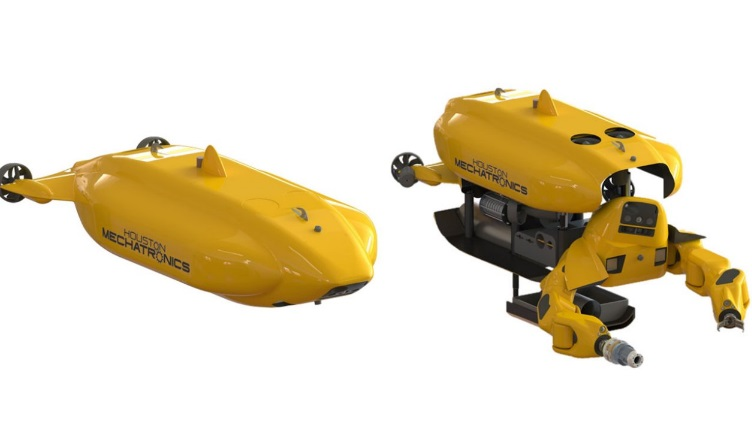
\includegraphics[scale=0.4]{submarine_robot}
		\caption{Houston Mechatronics's Aquanaut}
		\label{fig:aquanaut} 
	\end{figure}
	\item legged humanoid or animal-like robots for service missions;
	\begin{figure}[h!]
		\centering 
		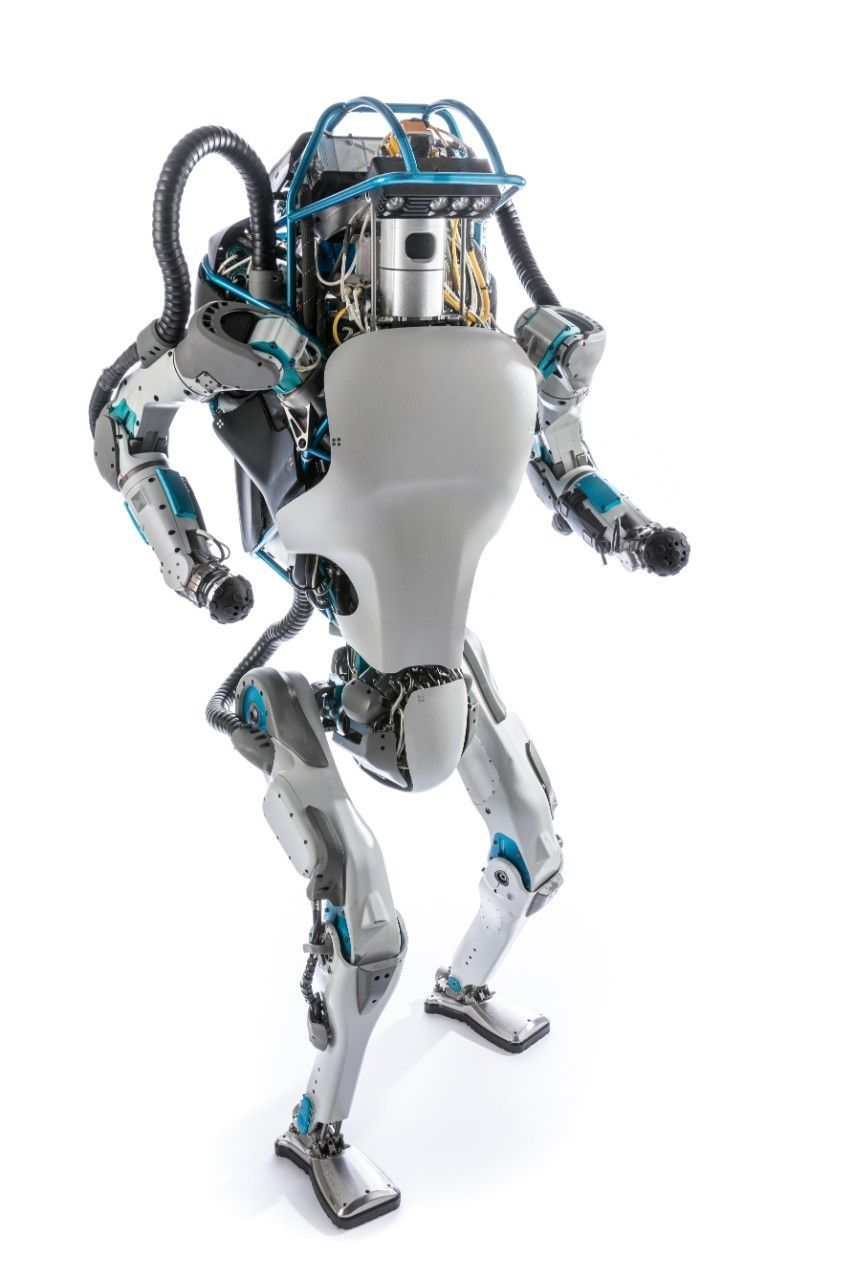
\includegraphics[scale=0.15]{atlas}
		\label{fig:atlas} 
		\quad
		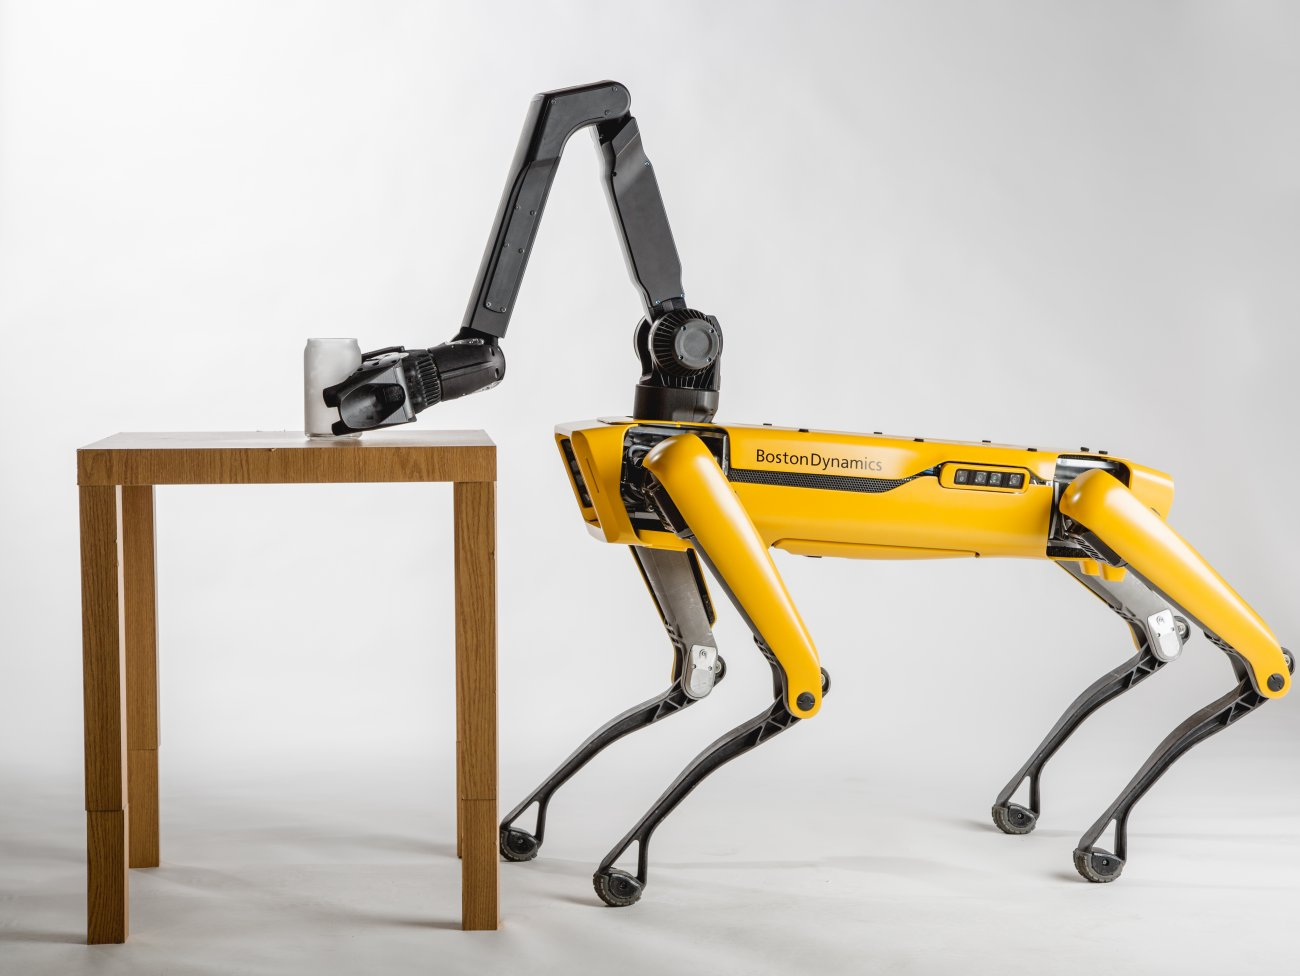
\includegraphics[scale=0.15]{spot_mini}
		\label{fig:spotmini} 
		\caption{Boston Dynamics's Atlas and Spot Mini}
	\end{figure}
	\item The most popular ones are the wheeled mobile manipulators or WMM, which combine a wheeled mobile base and one or more robotic arms.
	\begin{figure}[h!]
		\centering
		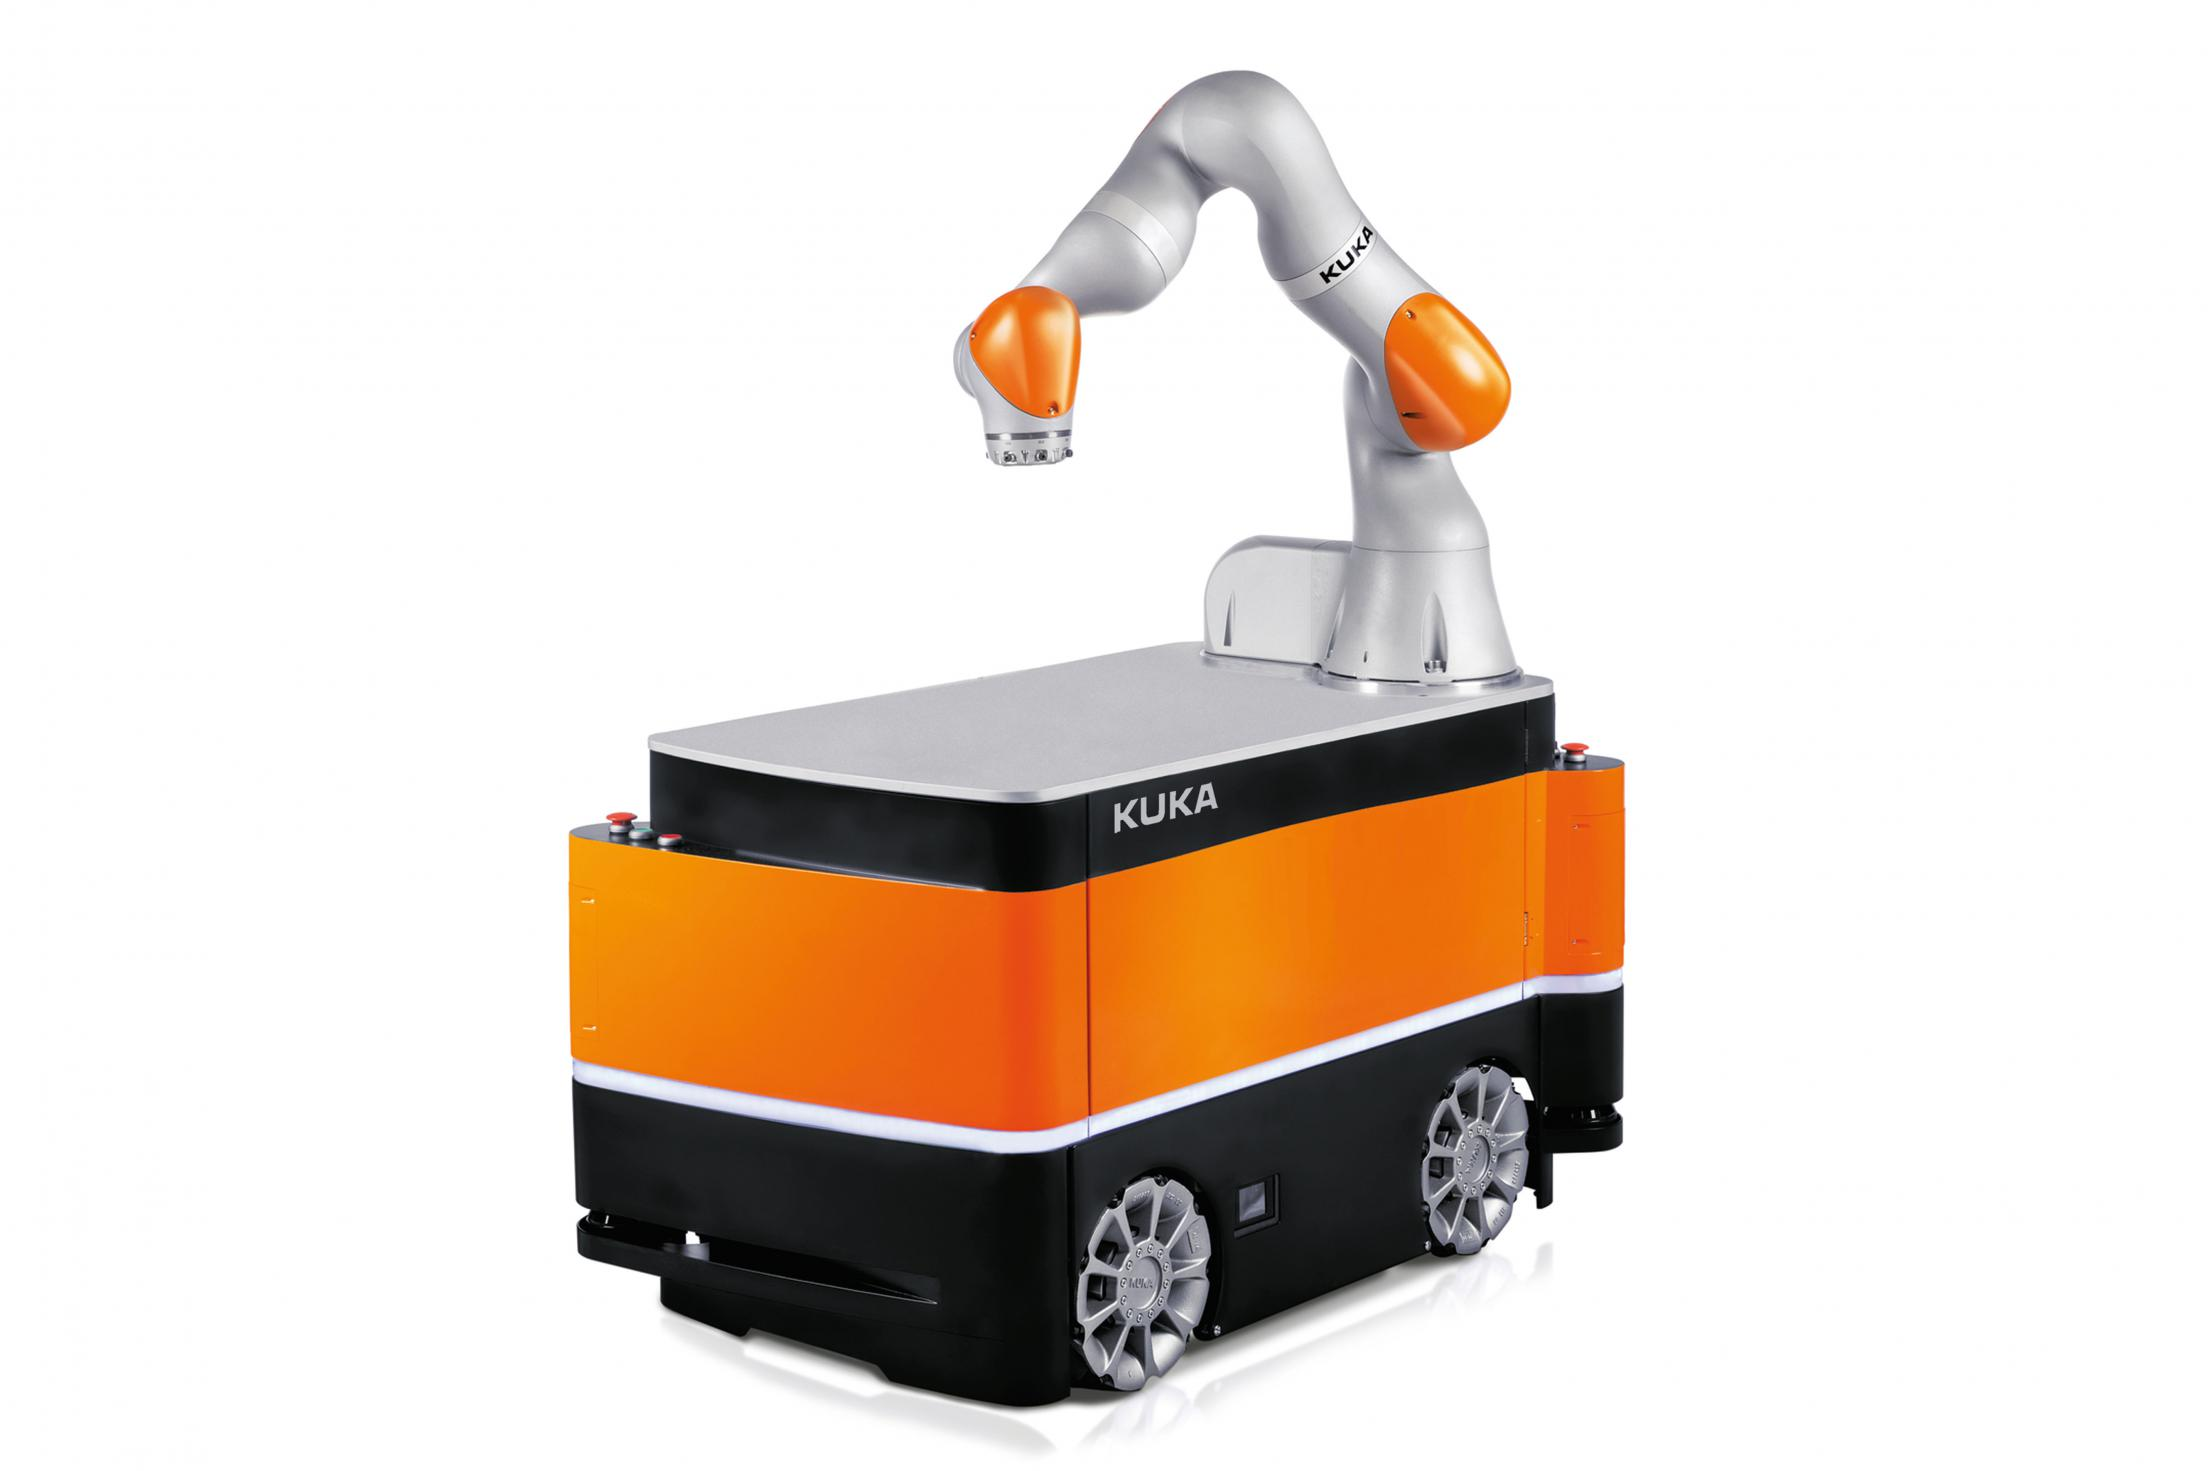
\includegraphics[scale=0.15]{kuka_iiwa}
		\caption{Kuka KMR iiwa}
		\label{fig:iiwa} 
	\end{figure}
\end{itemize}
Among the wheeled mobile manipulators there are many different types, but usually they have the following characteristics:
\begin{enumerate}
	\item The mobile base is a nonholonomic system;
	\item The entire system is often kinematically redundant with respect to the task to be achieved;
	\item The dynamic properties of the base are very different from the manipultor ones.
\end{enumerate}
Since it is important for the understanding of the problem, the concept of Nonholonomy is now explained.

\subsection{Holonomic and Nonholonomic constraints}
Considering a system of $N$ rigid bodies and assuming that all of them can reach any position in the space, in order to find uniquely the position of all the points of the system, it is necessary to define a vector of $6N = m$ parameters. This set of parameters is termed \textit{ generalized coordinates of the unconstrained system}. 
Constraints acting on the position (configuration) of the system are said to be  \textit{holonomic}. 
Holonomic constraints are expressed in the form:
\begin{equation}
h\left( x,q \right) =0
\end{equation}
where $h$ is a vector of dimension $s<m$.
The constraints that constrain the velocities of the system of rigid bodies but not their positions are called \textit{nonholonomic}. In general all constraints which are nonintegrable are said to be nonholonomic, so also inequality constraints about the configuration are considered nonholonomic. 
Nonholonomic constraints reduce the mobility of the mechanical system in a completely different way with respect to holonomic constraints. The fact that the constraint is nonintegrable means that there is no loss of accessibility to the all configuration space for the system. In other words, while the number of DOFs decreases due to the constraint, the number of generalized coordinates cannot be reduced, not even locally. Only the subspace of the generalized velocities is reduced.
Nonholonomic constraints are expressed in the form:
\begin{equation}
h( x,\dot{x},q) =0
\end{equation}
where $h$ is a vector of dimension $s<m$.
On the assumption that $h$ has continuous and continuously differentiable components, and its Jacobian $ \frac{\partial h}{\partial x} $ has full rank, the constraints equations allow the elimination of $s$ out of $m$ coordinates of the system. With the remaining $ n = m - s $ coordinates it is possible to determine uniquely the configurations of the system satisfying the constraints. Such coordinates are the \textit{generalized coordinates of the constrained system}.\\
Kinematic constraints both holonomic or nonholonomic are usually written in the Pfaffian form, i.e. linearly with respect to the generalized velocities.
\begin{equation}
	a_i^T \left( q \right)\dot{q} =0 \qquad i=1,...,k<n 
\end{equation}
\begin{equation*} 
	A^T \left( q \right)\dot{q} =0  
\end{equation*}
Talking about mobile robots, wheels are by far the most common mechanism to achieve locomotion. Any wheeled vehicle is subject to kinematic constraints that reduce in general its local mobility, while leaving intact the possibility of reaching arbitrary configurations by appropriate manoeuvres.
The pure rolling constraint for a wheel is expressed in the Pfaffian form as 
\begin{equation} 
	\dot{x}\sin\theta-\dot{y}\cos\theta=\left[
	\begin{matrix}
		\sin\theta & cos\theta & 0
	\end{matrix}
	\right] \dot{q}=0
\end{equation}
and entails that, in the absence of slipping, the velocity of the contact point has zero component in the direction orthogonal to the sagittal plane. The angular velocity of the disk around the vertical axis instead is unconstrained.
This constraint is nonholonomic, because it implies no loss of accessibility in the configuration space of the disk.

